\chapter{Methodology Chapter}


\section{Introduction}

Agile is not a methodology but more of an alternative to the existing SDLC Models. To articulate the methods and techniques used in this plan. In figure \ref{fig:agile} is the outcome after reviewing various SDLC methodologies with reference to \cite{TP-16}:
\begin{itemize}
	\item Adoption of the Agile Model.
	\item Suits the requirements for this project.
	\item Widely accepted within companies within the IT industry.
	\item Valuable learning curve in gaining experience with this model.
	\item Model has the ability to adapt and tailor itself within each increment as the project moves forward.
	\item Advantageous to the project.
\end{itemize}

\begin{figure}[Htbp]
\center 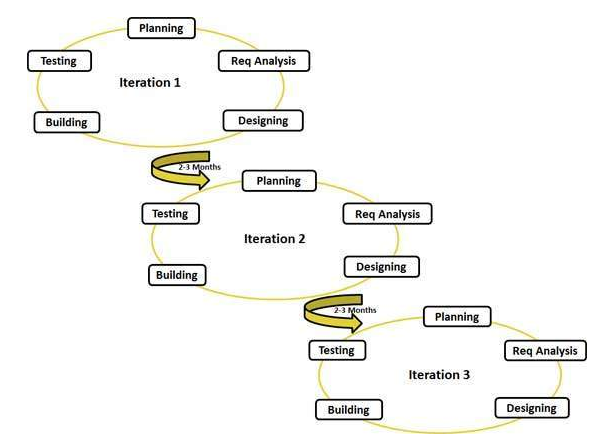
\includegraphics[width=400pt]{Figures/sdlc_agile_model}\\
\caption{Graphical illustration of the Agile Model \citep{TP-16}} \label{Figure: Graphical illustration of the Agile Model}
\label{fig:agile}
\end{figure}	

\subsection{What is Agile?}
Agile is an iterative approach to software delivery that builds software incrementally from the start of the project, instead of trying to deliver it all at once near the end. It works by breaking projects down into little bits of user functionality called user stories, prioritizing them, and then continuously delivering them in short two week cycles called iterations.

\begin{figure}[htbp]
\center 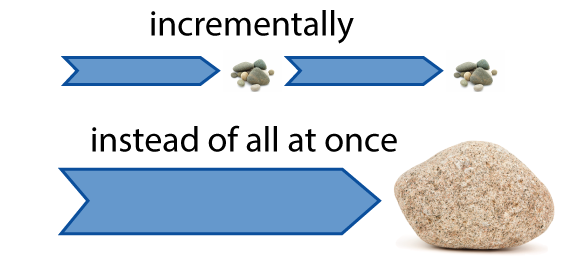
\includegraphics[width=400pt]{figures/incrementally-over-all-at-once}\\
\caption{Increments of the Agile Model \citep{AIAN-16}} \label{Figure: Increments of the Agile Model}
\label{fig:agile}
\end{figure}

\begin{figure}[htbp]
\center 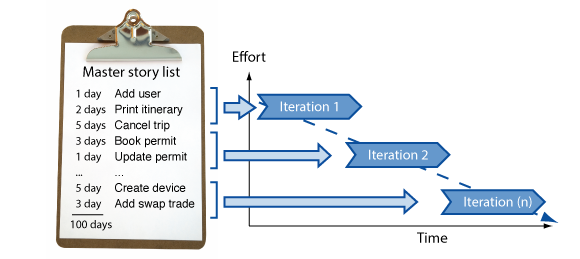
\includegraphics[width=400pt]{figures/burn-down-simple}\\
\caption{Iterations of the Agile Model \citep{AIAN-16}} \label{Figure: Iterations of the Agile Model}
\label{fig:agile}
\end{figure}

\subsection{How does it work?}
At its core, Agile does the same thing you and I do when faced with too much to do and not enough time. Then, using Agile estimation techniques, you size your stories relatively to each other, coming up with a guess as to how long you think each user story will take. Like most lists, there always seems to be more to do than time allows. So you ask your customer to prioritize their list so you get the most important stuff done first, and save the least important for last. Then you start delivering some value. You start at the top. Work your way to the bottom. Building, iterating, and getting feedback from your customer as you go. Then, as you and your customer starting delivering, one of two things is going to happen. You'll discover:

    You're going fast enough. All is good. Or,
    You have too much to do and not enough time.

At this point you have two choices. You can either a) do less and cut scope (recommended). Or you can b) push out the date and ask for more money.

\begin{figure}[htbp]
\center 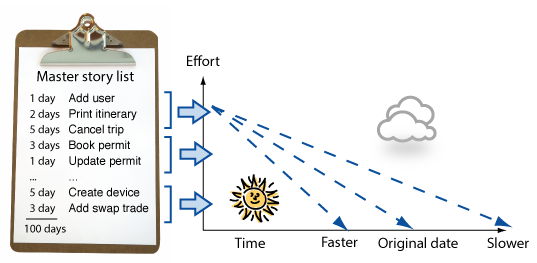
\includegraphics[width=400pt]{figures/update-the-plan}\\
\caption{Making a list \citep{AIAN-16}} \label{Figure: Making a list}
\label{fig:agile}
\end{figure}

\subsection{How is it different?}
Analysis, design, coding, and testing are continuous activities

You are never done analysis, design, coding and testing on an Agile project. So long as there are features to build, and the means to deliver them, these activities continue for the duration of the project.

\subsection{Agile vs Waterfall}
Traditional Waterfall treats analysis, design, coding, and testing as discrete phases in a software project. This worked OK when the cost of change was high. But now that it's low it hurts us in a couple of ways. First off, when the project starts to run out of time and money, testing is the only phase left. This means good projects are forced to cut testing short and quality suffers. Secondly, because working software isn't produced until the end of the project, you never really know where you are on a Waterfall project. That last 20\% of the project always seems to take 80\% of the time.

\section{Data Collection Methods}

\subsection{Internet Search}
Discusses where I obtained my information
\subsection{Supervisor Input}
Discussion on how to store the encrypted data in tables 
\subsection{Journals in Library}
Journals which were read and relevant to this project


\section{Method of Analysis}

\subsection{Formulation of Where to Start}
Researching the title of the project
\subsection{Early System Implementation}
This project was linked to an assignment which helped in my progression
\subsection{Review of Literature}
Undertaking a literature review aided with making comparisons of other systems produced


\section{Summary}

Summary with all terms discussed within the chapter
\begin{comment}
\subsection{Subsection header 1}
fdsdfsdfds
\subsection{Subsection header 2}
fdsdfsdfds
\subsection{Subsection header 3}
fdsdfsdfds
\end{comment}
